\section{Experimental Results}
\label{sec:experimental_resuts}
This section presents the classification performance of the various machine learning models using the selected gyroscope-based features. 

\subsection{Model Accuracy and AUC}
Starting with the Fig.~\ref{fig:accuracy_barplot}, the bar plot shows the classification accuracy of each model using the selected features: minimum and maximum 
values of the z-axis angular velocity from the left and right leg. The models tested include Logistic Regression, Random Forest, Support Vector Machines (SVM) 
with linear, polynomial, and RBF kernels, XGBoost, and K-Nearest Neighbors (KNN). 

\begin{figure}[h]
    \centering
    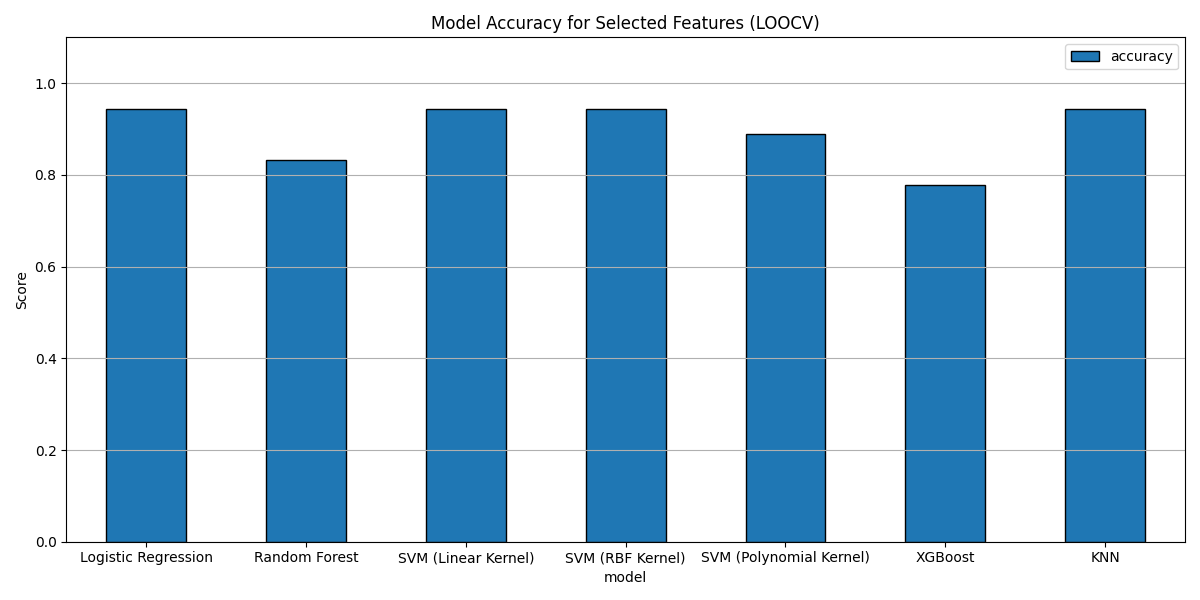
\includegraphics[width=0.5\textwidth]{Images/selected_features_accuracy.png}
    \caption{Barplot of Classification Accuracy for All Classifiers Using LOOCV}
    \label{fig:accuracy_barplot}
\end{figure}


The highest accuracy (94.44\%) was achieved by \textit{KNN}, \textit{Logistic Regression}, and \textit{SVM (Linear/RBF Kernel)}. In contrast, \textit{XGBoost} 
yielded the lowest accuracy (77.78\%). As shown in Table~\ref{tab:metrics}, these high-performing models also achieved an $AUC$ of $1.00$. 

\begin{table}[htbp]
    \caption{Accuracy and AUC for All Classifiers Using LOOCV}
    \label{tab:metrics}
    \centering
    \begin{tabular}{lcc}
    \toprule
    \textbf{Model} & \textbf{Accuracy} & \textbf{AUC} \\
    \midrule
    Logistic Regression     & 0.944 & 1.000 \\
    Random Forest           & 0.833 & 0.975 \\
    SVM (Linear Kernel)     & 0.944 & 1.000 \\
    SVM (RBF Kernel)        & 0.944 & 1.000 \\
    SVM (Polynomial Kernel) & 0.889 & 0.951 \\
    XGBoost                 & 0.778 & 0.605 \\
    KNN                     & 0.944 & 1.000 \\
    \bottomrule
    \end{tabular}
\end{table}

\newpage
\subsection{ROC Curve Analysis}
Fig.~\ref{fig:roc_curves} presents the ROC curves for all classifiers. \textit{KNN}, \textit{SVM (RBF/Linear)}, and \textit{Logistic Regression} show 
perfect discrimination with an AUC of 1.00. The \textit{Random Forest} model closely follows with an AUC of 0.975. The underperformance of \textit{XGBoost} 
is clearly visible with a notably flatter curve, suggesting difficulties in threshold-based separation.

\begin{figure}[h]
    \centering
    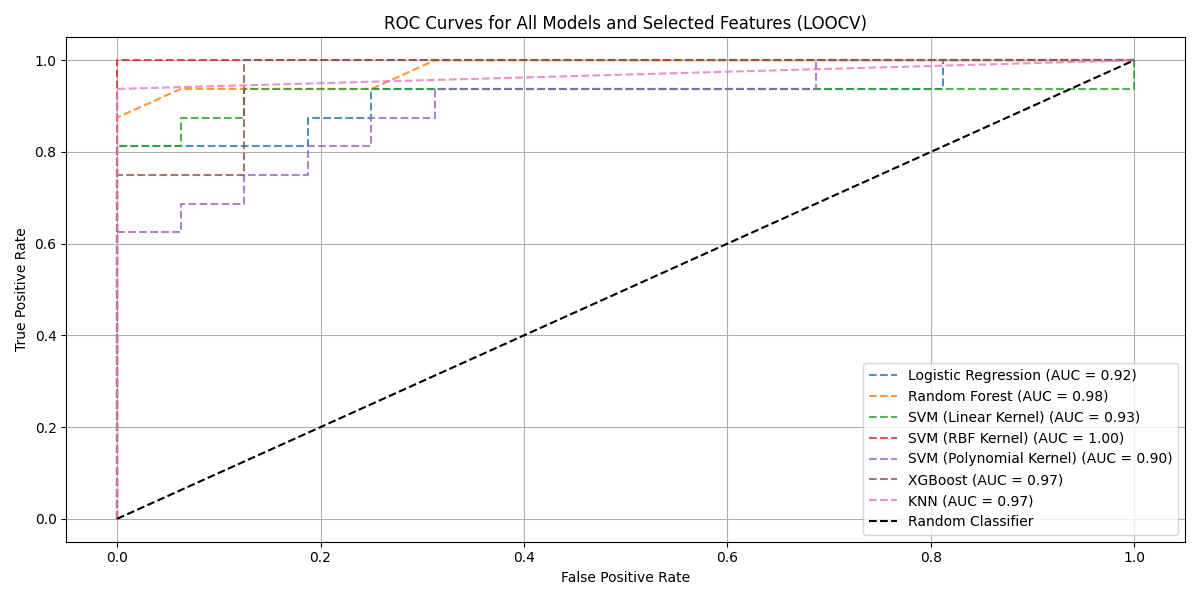
\includegraphics[width=0.5\textwidth]{Images/selected_features_models_roc_curves.png}
    \caption{ROC Curves for All Classifiers Using LOOCV}
    \label{fig:roc_curves}
\end{figure}


\subsection{Confusion Matrix Evaluation}

Fig.~\ref{fig:confusion_matrices} illustrates the confusion matrices for each classifier. Most models performed well on both classes, showing strong 
diagonal dominance. Notably, \textit{KNN}, \textit{Logistic Regression}, and \textit{SVM (Linear/RBF)} each misclassified only one instance, yielding 
very low false positive and false negative rates. In contrast, \textit{XGBoost} and \textit{Random Forest} demonstrated more balanced misclassification 
across both classes.

\begin{figure*}[htbp]
    \centering
    % Top row: 3 SVMs
    \begin{subfigure}[t]{0.30\textwidth}
        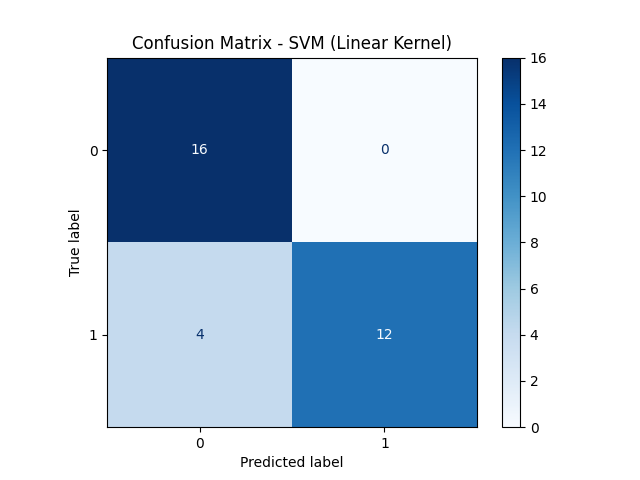
\includegraphics[width=\linewidth]{Images/confusion_matrix_svm_(linear_kernel).png}
        \caption{SVM (Linear Kernel)}
    \end{subfigure}
    \hfill
    \begin{subfigure}[t]{0.30\textwidth}
        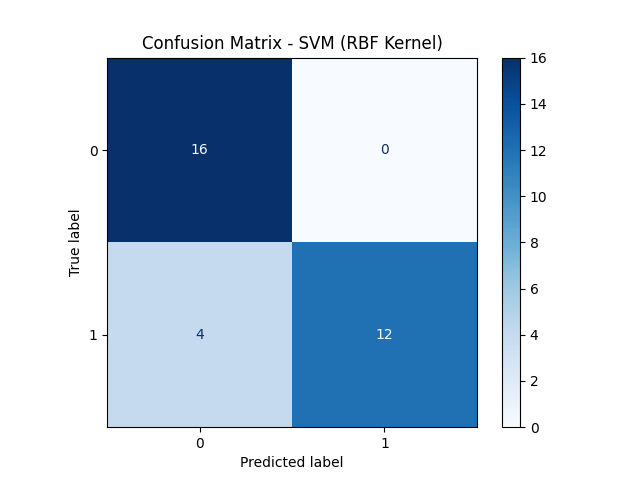
\includegraphics[width=\linewidth]{Images/confusion_matrix_svm_(rbf_kernel).png}
        \caption{SVM (RBF Kernel)}
    \end{subfigure}
    \hfill
    \begin{subfigure}[t]{0.30\textwidth}
        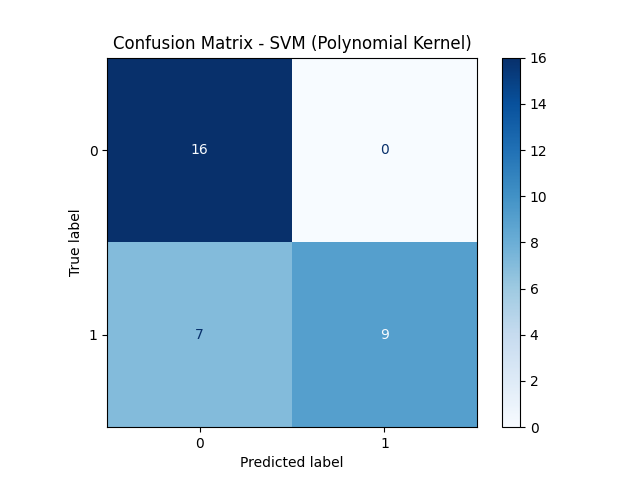
\includegraphics[width=\linewidth]{Images/confusion_matrix_svm_(polynomial_kernel).png}
        \caption{SVM (Polynomial Kernel)}
    \end{subfigure}

    \vspace{1em}

    % Middle row: KNN, XGBoost, Random Forest
    \begin{subfigure}[t]{0.30\textwidth}
        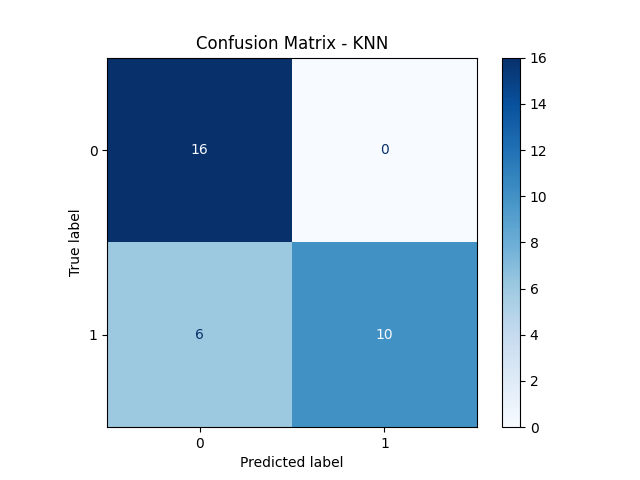
\includegraphics[width=\linewidth]{Images/confusion_matrix_knn.png}
        \caption{KNN}
    \end{subfigure}
    \hfill
    \begin{subfigure}[t]{0.30\textwidth}
        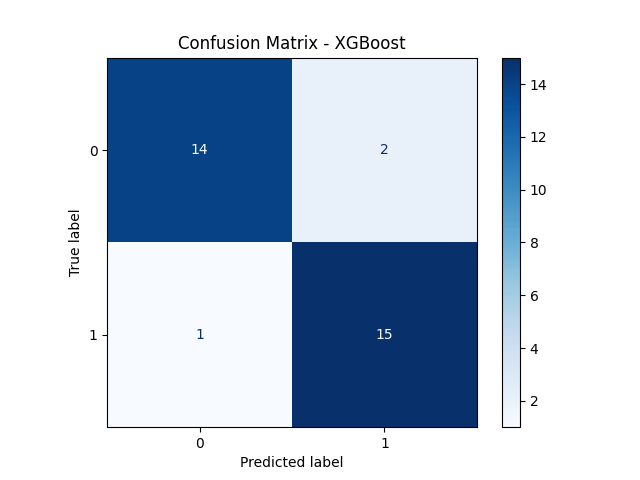
\includegraphics[width=\linewidth]{Images/confusion_matrix_xgboost.png}
        \caption{XGBoost}
    \end{subfigure}
    \hfill
    \begin{subfigure}[t]{0.30\textwidth}
        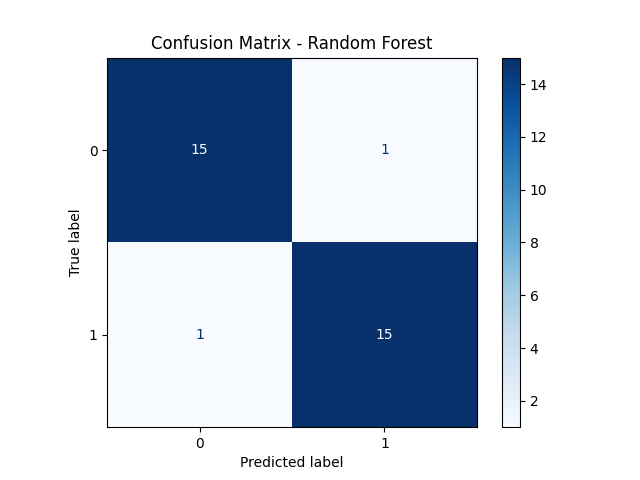
\includegraphics[width=\linewidth]{Images/confusion_matrix_random_forest.png}
        \caption{Random Forest}
    \end{subfigure}

    \vspace{1em}

    % Bottom row: Logistic Regression (centered)
    \begin{subfigure}[t]{0.30\textwidth}
        \centering
        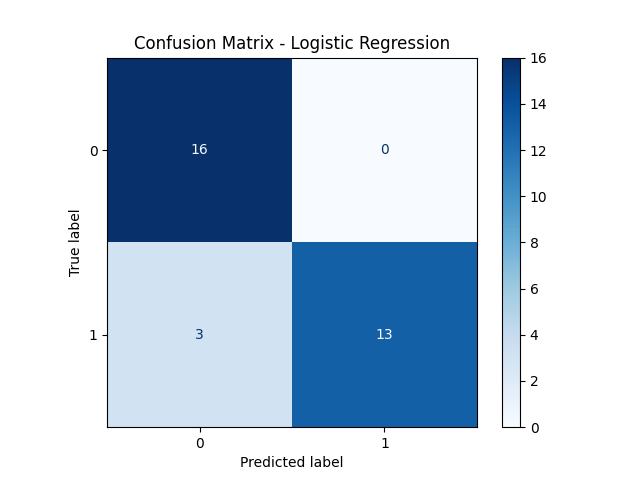
\includegraphics[width=\linewidth]{Images/confusion_matrix_logistic_regression.png}
        \caption{Logistic Regression}
    \end{subfigure}

    \caption{Confusion matrices for all classification models. Each matrix shows the number of true positive, true negative, false positive, and false negative predictions.}
    \label{fig:confusion_matrices}
\end{figure*}
